\begin{frame}[label=title]
    \centering
    \begin{figure}[H]
        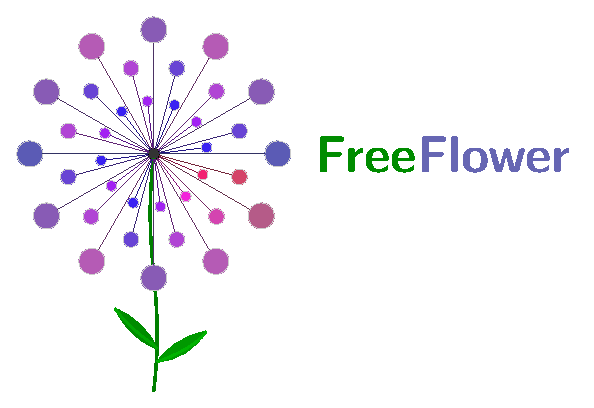
\includegraphics[keepaspectratio, width=0.7\paperwidth, height=\paperheight]{Logos/FreeFlower.pdf}
    \end{figure}
    Informatik: Data Science und Sicherheit\\
    \emoji{clamp}\textbf{Kompression}: Maximale Balance
\end{frame}

\begin{frame}{Kodierung der \textbf{maximalen Häufigkeit}}
	\only<1->{	\textbf{Idee}: Summe der Buchstabenhäufigkeiten im linken und rechten Teilbaum ausbalancieren\\[.5cm]}
	
	\only<2>{\textbf{Beispiel}:
		\begin{table}[H]
			\centering
			\begin{tabular}{c|c|c|c|c|c|c}
				\textbf{Buchstabe} & \textbf{A} & \textbf{B} & \textbf{C} & \textbf{D}& \textbf{E}& \textbf{F} \\\midrule\midrule
				Relative Häufigkeit & 25\% & 25\% & 13\% & 13\%& 12\%& 12\%
			\end{tabular}
		\end{table}}
\end{frame}

\begin{frame}{Kodierung der \textbf{maximalen Häufigkeit}: Beispiel}
	\scriptsize{
	\begin{table}[H]
		\centering
		\begin{tabular}{c|c|c|c|c|c|c}
			\textbf{Buchstabe} & \textbf{A} & \textbf{B} & \textbf{C} & \textbf{D}& \textbf{E}& \textbf{F} \\\midrule\midrule
			Relative Häufigkeit & 25\% & 25\% & 13\% & 13\%& 12\%& 12\%
		\end{tabular}
		\end{table}}
	\centering
	\begin{tikzpicture}
		[-,>=stealth',
		level distance=18mm,
		level 1/.style={sibling distance=60mm},
		level 2/.style={sibling distance=30mm},
		level 3/.style={sibling distance=15mm},
		level 4/.style={sibling distance=8mm},
		leaf/.style={circle, draw},
		label/.style={red},
		edge from parent path={(\tikzparentnode.south) -- (\tikzchildnode)}] 
		
		
		\usetikzlibrary{shapes}
		\tikzstyle{n} = [text width=1cm,align=center]
		\tikzstyle{r} = [text=red]
		
		\node[n]{\textcolor{BlueGreen}{A,B,C,D,E,F}\\ 100\%}[edge from parent]
		child {node[n] {\textcolor{BlueGreen}{A,B}\\ 50\%}
			child {node[n, visible on=<2->] {\textcolor{BlueGreen}{A}\\ 25\%\\\textcolor{red}{00}}
				edge from parent[visible on=<2->] node[left,r]{0};
			}
			child {node[n, visible on=<2->] {\textcolor{BlueGreen}{B}\\ 25\%\\\textcolor{red}{01}}
				edge from parent[visible on=<2->] node[r,right]{1};
			}
			edge from parent node[left,r]{0};
		}
		child {node[n]{\textcolor{BlueGreen}{C,D,E,F}\\ 50\%}
			child {node[n, visible on=<3->] {\textcolor{BlueGreen}{C,E}\\ 25\%}
				child {node[n, visible on=<4->] {\textcolor{BlueGreen}{C}\\ 13\%\\\textcolor{red}{100}}
					edge from parent[visible on=<4->] node[left,r]{0};
				}
				child {node[n, visible on=<4->] {\textcolor{BlueGreen}{E}\\ 12\%\\\textcolor{red}{101}}
					edge from parent[visible on=<4->] node[r,right]{1};
				}
				edge from parent[visible on=<3->] node[left,r]{0};
			}
			child {node[n, visible on=<3->] {\textcolor{BlueGreen}{D,F}\\ 25\%}
				child {node[n, visible on=<5->] {\textcolor{BlueGreen}{D}\\ 13\%\\\textcolor{red}{110}}
					edge from parent[visible on=<5->] node[left,r]{0};
				}
				child {node[n, visible on=<5->] {\textcolor{BlueGreen}{F}\\ 12\%\\\textcolor{red}{111}}
					edge from parent[visible on=<5->] node[r,right]{1};
				}
				edge from parent[visible on=<3->] node[r,right]{1};
			}
			edge from parent node[r,right]{1};
		};
	\end{tikzpicture}
\end{frame}
 
\begin{frame}{Kodierung der \textbf{maximalen Häufigkeit}}
	\textbf{Problem}: Was passiert bei folgender Verteilung?
		\begin{table}[H]
			\centering
			\begin{tabular}{c|c|c|c|c|c|c}
				\textbf{Buchstabe} & \textbf{A} & \textbf{B} & \textbf{C} & \textbf{D}& \textbf{E}& \textbf{F} \\\midrule\midrule
				Relative Häufigkeit & 49\% & 1\% & 25\% & 8\%& 9\%& 8\%
			\end{tabular}
	\end{table}
\end{frame}

\begin{frame}{Kodierung der \textbf{maximalen Häufigkeit}: Problem}
	\scriptsize{
		\begin{table}[H]
			\centering
						\begin{tabular}{c|c|c|c|c|c|c}
				\textbf{Buchstabe} & \textbf{A} & \textbf{B} & \textbf{C} & \textbf{D}& \textbf{E}& \textbf{F} \\\midrule\midrule
				Relative Häufigkeit & 49\% & 1\% & 25\% & 8\%& 9\%& 8\%
			\end{tabular}
	\end{table}}
	\centering
	\begin{tikzpicture}
		[-,>=stealth',
		level distance=15mm,
		level 1/.style={sibling distance=60mm},
		level 2/.style={sibling distance=30mm},
		level 3/.style={sibling distance=15mm},
		level 4/.style={sibling distance=15mm},
		level 5/.style={sibling distance=15mm},
		leaf/.style={circle, draw},
		label/.style={red},
		edge from parent path={(\tikzparentnode.south) -- (\tikzchildnode)}] 
		
		
		\usetikzlibrary{shapes}
		\tikzstyle{n} = [text width=1cm,align=center]
		\tikzstyle{r} = [text=red]
		
		\node[n]{\textcolor{BlueGreen}{A,B,C,D,E,F}\\ 100\%}[edge from parent]
		child {node[n] {\textcolor{BlueGreen}{A,B}\\ 50\%}
			child {node[n, visible on=<2->] {\textcolor{BlueGreen}{A}\\ 49\%\\\textcolor{red}{00}}
				edge from parent[visible on=<2->] node[left,r]{0};
			}
			child {node[n, draw, visible on=<2->] {\textcolor{BlueGreen}{B}\\ 1\%\\\textcolor{red}{01}}
				edge from parent[visible on=<2->] node[r,right]{1};
			}
			edge from parent node[left,r]{0};
		}
		child {node[n]{\textcolor{BlueGreen}{C,D,E,F}\\ 50\%}
			child {node[n, visible on=<3->] {\textcolor{BlueGreen}{C}\\ 25\%\\\textcolor{red}{10}}
				edge from parent[visible on=<3->] node[left,r]{0};
			}
			child {node[n, visible on=<3->] {\textcolor{BlueGreen}{D,E,F}\\ 25\%}
				child {node[n, draw, visible on=<4->] {\textcolor{BlueGreen}{E}\\ 9\%\\\textcolor{red}{110}}
					edge from parent[visible on=<4->] node[r,left]{0};
				}
				child {node[n, visible on=<4->] {\textcolor{BlueGreen}{D,F}\\ 16\%\\}
					child {node[n, draw, visible on=<5->] {\textcolor{BlueGreen}{D}\\ 8\%\\\textcolor{red}{1110}}
						edge from parent[visible on=<5->] node[left,r]{0};
					}
					child {node[n, draw, visible on=<5->] {\textcolor{BlueGreen}{F}\\ 8\%\\\textcolor{red}{1111}}
						edge from parent[visible on=<5->] node[right,r]{1};
					}
					edge from parent[visible on=<4->] node[right,r]{1};
				}
				edge from parent[visible on=<3->] node[r,right]{1};
			}
			edge from parent node[r,right]{1};
		};
	\end{tikzpicture}
\end{frame}

\begin{frame}[label=auftrag]{Auftrag}
	\begin{itemize}
		\item \aufgabebox{Aufgabe 1.3, 1.5}
		\item \challengebox{Aufgaben 1.4}
	\end{itemize}
\end{frame}
